\documentclass{utmreport}
\newcommand{\ReportTitle}{Cryptanalysis of Monoalphabetic Ciphers}
\newcommand{\ReportSubtitle}{\ReportCourse: frequency analysis and substitution recovery}
% Load after defining ReportTitle; optional per-report settings follow below.
% Shared identity and course details for all laboratory reports.
\student{Gafenco Victor}{FAF-241}
\supervisor{asist. univ. Zaica Maia}{}
\newcommand{\ReportCourse}{Cryptography}
\cityyear{Chișinău}{2026}
\institution{Technical University of Moldova}
\faculty{Faculty of Computers, Informatics, and Microelectronics}
\department{Department of Software Engineering}
\studyprogramme{Software Engineering Study Programme}
\newcommand{\repositoryurl}{https://github.com/yoda-dinmd/crypt-labs}

\providecommand{\ReportNumber}{\expandafter\ReportNumberFromJob\jobname\relax}
\def\ReportNumberFromJob#1#2#3#4\relax{#4}
\providecommand{\ReportSubtitle}{}
\selectlanguage{english}
\ifPDFTeX\else\setmonofont{Liberation Mono}\fi
\utmlogo{../latex/assets/UTM_Logo_English.jpeg}
\documenttype{Laboratory report no. \ReportNumber}
\reporttitle{\ReportTitle}
\reportsubtitle{\ReportSubtitle}
\hypersetup{
  pdftitle={\ReportTitle},
  pdfauthor={\UTMStudentName},
  pdfsubject={\ReportCourse{} laboratory report no. \ReportNumber}
}

% Shared wording for references to the supplied Cryptography handouts.
% Arguments: laboratory number, topic, optional descriptive text (including punctuation).
\newcommand{\ReportHandoutReference}[3]{%
  \textit{Laboratory Work No. #1. #2}. Supplied course handout#3}

\setcounter{tocdepth}{1}
\lstset{language={},literate={—}{{\textemdash}}1 {•}{{\textbullet}}1}
\begin{document}
\makeutmreporttitlepage
\tableofcontents
\clearpage
\begin{utmabstract}[Abstract]
This laboratory examines the recovery of an English message encrypted with a monoalphabetic substitution. Letter frequencies provide initial hypotheses, while repeated words, common letter combinations and grammatical context constrain the remaining substitutions. The report reconstructs a 19-step analysis of Variant 1, supported by four supplied frequency screenshots. The cryptogram contains 2,567 letters and 25 distinct ciphertext symbols. All observed symbols are resolved consistently; the final unused alphabet pair is inferred by elimination. Intermediate extracts illustrate the gradual recovery of the passage, and the complete ciphertext and literal plaintext are preserved for comparison. The result demonstrates that a large substitution key space does not conceal the statistical structure of natural language.
\par\utmkeywords{cryptanalysis, substitution, frequency analysis, word patterns, plaintext recovery}
\end{utmabstract}
\utmintroduction
The objective is to recover an English plaintext from a monoalphabetic cryptogram. The attack uses the frequency analysis method described in the laboratory handout \cite{handout}. Only letters are encrypted; numbers, spaces and punctuation provide additional information. The required report explains the successive deductions, as in the handout's worked example.

Variant 1 is used to match the supplied reference report by Gabriel Balan \cite{reference}. Its four frequency screenshots and deduction sequence are reused with attribution. The analysis below reconstructs the substitutions and verifies them against the Variant 1 ciphertext in the handout. Intermediate extracts are reconstructed text, not new captures of an interactive session. This laboratory requires a report only and contains no application implementation.

The report follows the structure of Laboratory Work No. 1: theoretical background, practical analysis, results and conclusions. Complete source and result texts are included in the appendices. The focus is on explaining why each proposed substitution is plausible and how it fits the rest of the message.

\chapter{Short theory}
A fixed substitution changes the labels of letters while preserving much of the structure that makes a language recognizable. The following properties form the basis of the attack described in the handout \cite{handout}.
\section{Monoalphabetic substitution}
Let $A$ be the 26-letter English alphabet and let $\pi$ be a permutation of $A$. For plaintext letter $p_i$ and ciphertext letter $c_i$, encryption and decryption are:
\begin{equation}
c_i=\pi(p_i),\qquad p_i=\pi^{-1}(c_i).
\end{equation}
The same plaintext letter always produces the same ciphertext symbol. Consequently, letter counts, repeated-letter patterns and word lengths survive encryption. A general substitution has $26!\approx4.03\times10^{26}$ possible keys, but this large key space does not prevent an attack based on language patterns. Unlike brute force, frequency analysis tries to infer the permutation from the message itself.

\section{Letter frequencies}
For a ciphertext of $N$ alphabetic characters, the relative frequency of symbol $c$ is:
\begin{equation}
f_C(c)=\frac{n_C(c)}{N}\times100\%,
\end{equation}
where $n_C(c)$ denotes its count. Uppercase and lowercase letters are counted together; digits, punctuation, spaces and line breaks are excluded. For a sufficiently long text, the distribution often resembles the average distribution of its language. English is used here because the assignment specifies an English plaintext.

Table~\ref{tab:english} reproduces the English reference values from the handout. They support initial guesses, not a unique key: topic and vocabulary can substantially change a particular message's distribution.
\clearpage
\begin{table}[!htbp]
\caption{English letter frequencies in percent, from the handout \cite{handout}}
\label{tab:english}\centering
\begin{tabular}{crcr}\hline
Letter & Frequency & Letter & Frequency\\\hline
A & 8.17 & N & 6.75\\ B & 1.49 & O & 7.51\\
C & 2.78 & P & 1.93\\ D & 4.25 & Q & 0.09\\
E & 12.70 & R & 5.99\\ F & 2.23 & S & 6.33\\
G & 2.01 & T & 9.06\\ H & 6.09 & U & 2.76\\
I & 6.97 & V & 0.98\\ J & 0.15 & W & 2.36\\
K & 0.77 & X & 0.15\\ L & 4.03 & Y & 1.97\\
M & 2.41 & Z & 0.07\\\hline
\end{tabular}
\end{table}

\section{Word patterns and consistency}
Common English digraphs (two-letter sequences) include TH, HE, AN, IN, ER and ON. Common trigraphs (three-letter sequences) include THE, AND, THA, ENT and ION. The ordinary one-letter words \textit{a} and \textit{i}, doubled letters and repeated short words also help constrain the key. For example, the partial pattern \texttt{tQe} strongly suggests \texttt{the}.

A useful hypothesis must explain several occurrences without contradicting earlier deductions. Each ciphertext symbol has one plaintext value, and different ciphertext symbols have different plaintext values. A guessed letter that produces one readable word but breaks several others should be reconsidered. Proper names and rare words become useful later, after common words have established most of the key.

\chapter{Practical analysis}
The practical work reconstructs the solution sequence in the supplied reference \cite{reference}. All mappings below run from ciphertext to plaintext: $V\rightarrow e$ means that ciphertext V represents plaintext e. In partial decryptions, unresolved symbols are uppercase and resolved letters are lowercase.

\section{Frequency evidence}
The supplied cryptogram contains 2,567 letters and uses 25 distinct ciphertext symbols. Ciphertext M does not occur. Figures~\ref{fig:cipherfreq} and~\ref{fig:englishfreq} show the ranked frequency tables extracted from the reference report. The integer counts in the ciphertext screenshot agree with the counts obtained from Variant 1 in the handout.
\begin{figure}[htbp]
\centering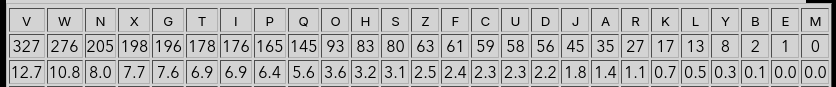
\includegraphics[width=\textwidth]{screenshots/ciphertext-frequency.png}
\caption{Ranked ciphertext frequencies, reused from the reference report \cite{reference}}\label{fig:cipherfreq}
\end{figure}
\begin{figure}[htbp]
\centering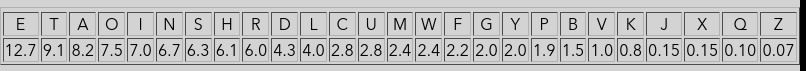
\includegraphics[width=\textwidth]{screenshots/english-frequency.png}
\caption{Ranked English frequencies, reused from the reference report \cite{reference}}\label{fig:englishfreq}
\end{figure}

Ciphertext V appears 327 times, giving $327/2567\times100\%\approx12.74\%$. Its frequency is close to the English reference of 12.70\% for e. Ciphertext W appears 276 times, approximately 10.75\%, and is a candidate for t. The screenshot rounds these values to 12.7\% and 10.8\%.

Ranking alone is insufficient. Ciphertext N is third with 205 occurrences, but represents o, whereas T is sixth with 178 occurrences and represents a. These substitutions must be established from words, rather than by matching two sorted lists mechanically.

\clearpage
The alphabetically ordered profiles in Figures~\ref{fig:englishprofile} and~\ref{fig:cipherprofile} illustrate the same statistical clues. The strongest English peaks occur at E and T; the strongest ciphertext peaks occur at V and W. These are separate distributions: the passage need not match average English exactly.
\begin{figure}[htbp]
\centering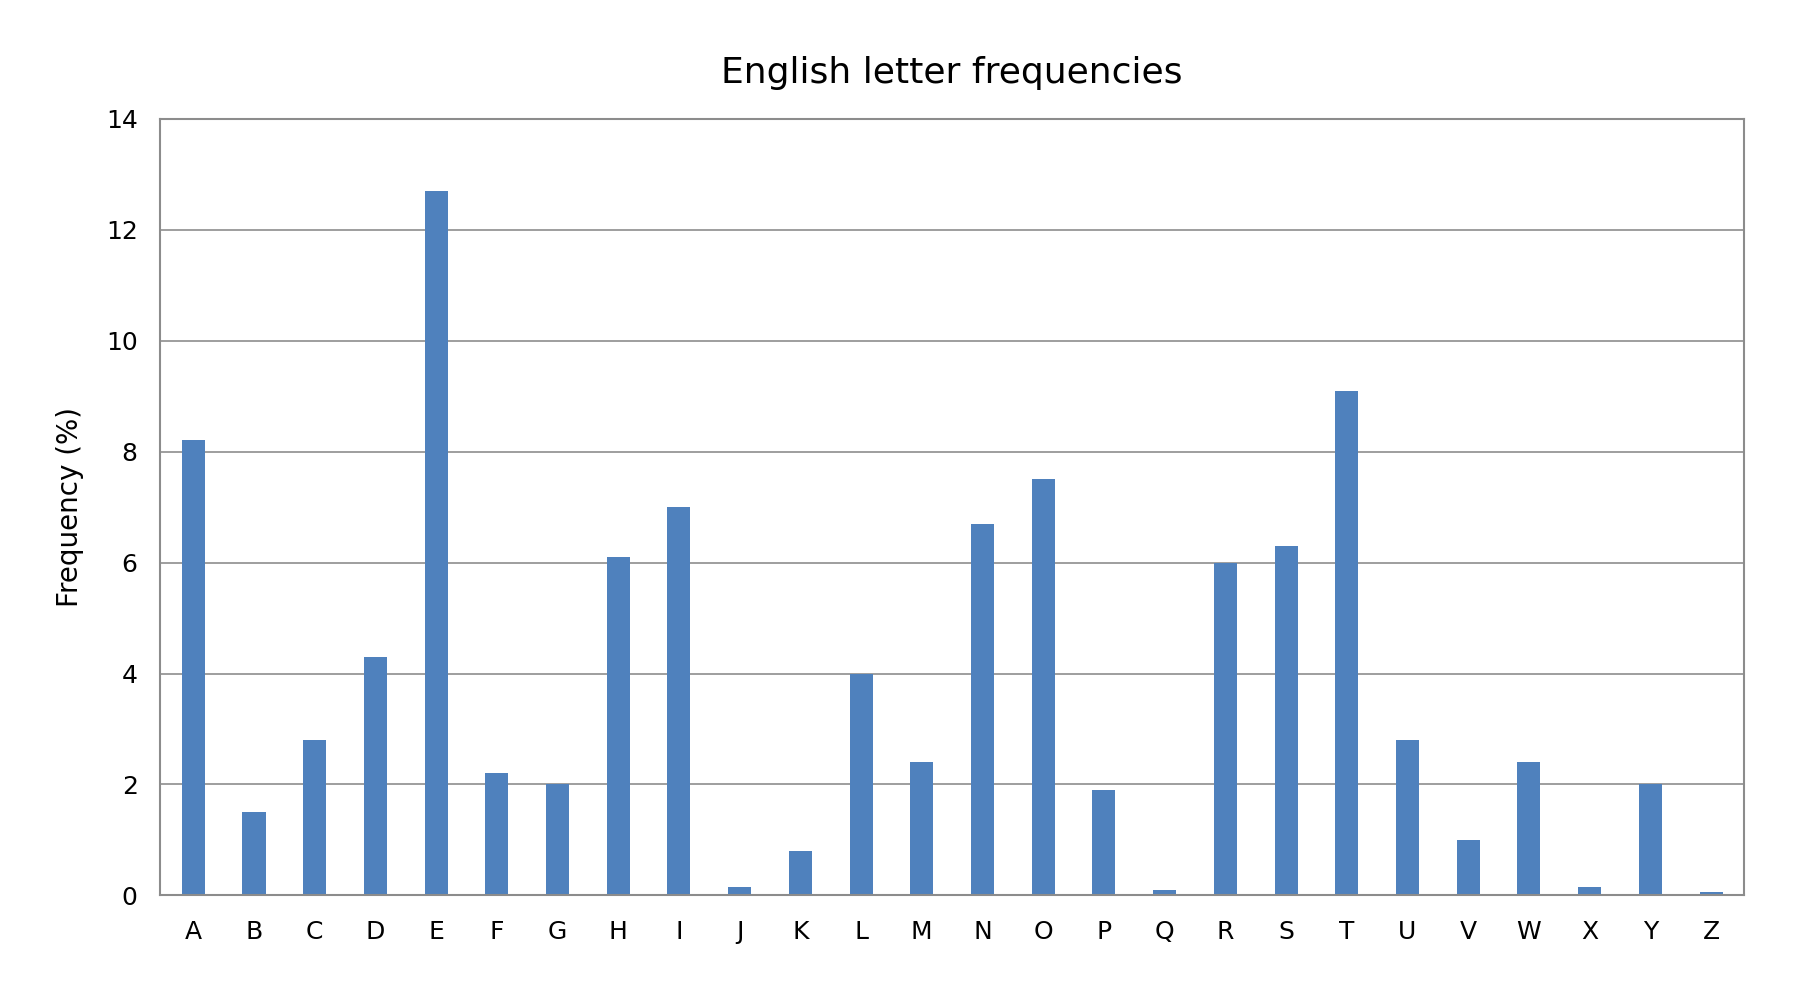
\includegraphics[width=0.78\textwidth]{screenshots/english-profile.png}
\caption{English frequency profile, reused from the reference report \cite{reference}}\label{fig:englishprofile}
\end{figure}
\begin{figure}[htbp]
\centering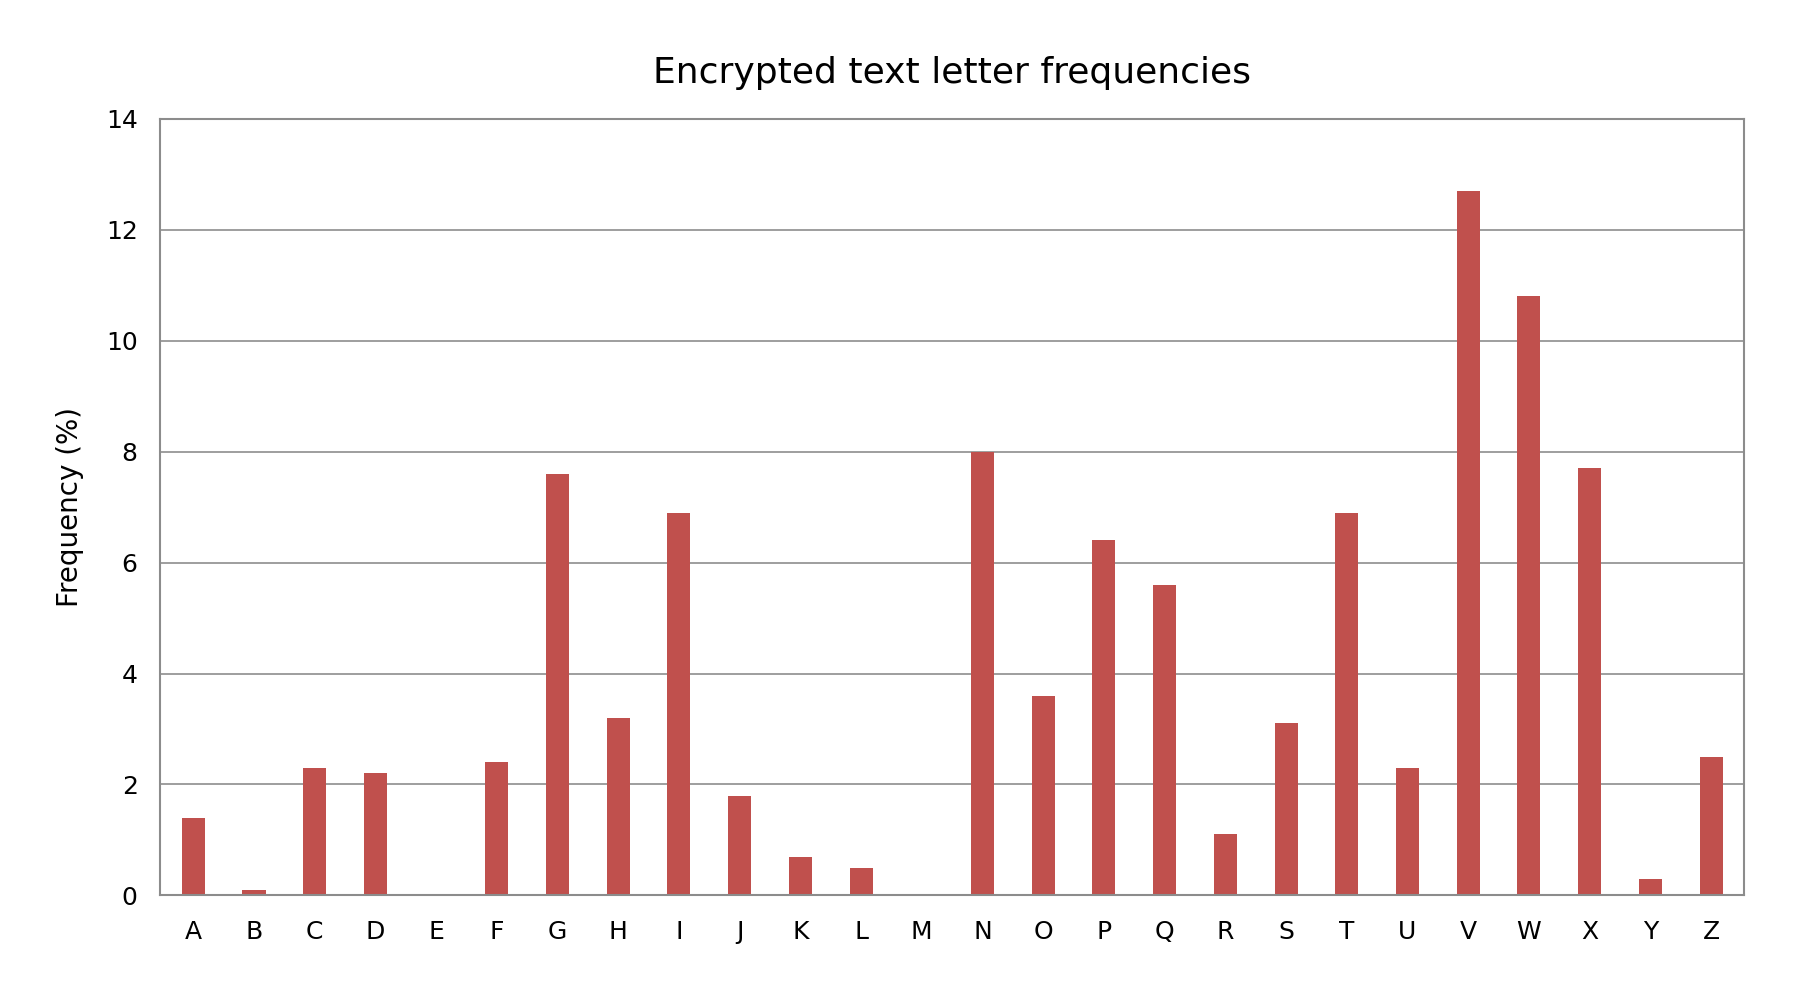
\includegraphics[width=0.78\textwidth]{screenshots/ciphertext-profile.png}
\caption{Ciphertext frequency profile, reused from the reference report \cite{reference}}\label{fig:cipherprofile}
\end{figure}
\clearpage
\section{Steps 1--7: common letters}
The first substitutions combine frequency hypotheses with short recurring words. The sequence follows the reference report \cite{reference}:
\begin{enumerate}
\item select $V\rightarrow e$: V occurs 327 times (12.74\%), making it the strongest candidate for the most frequent English letter;
\item select $W\rightarrow t$: W occurs 276 times (10.75\%); this second major peak suggests t, and the two replacements expose repeated instances of \texttt{tQe};
\item infer $Q\rightarrow h$: interpreting \texttt{tQe} as \texttt{the} confirms a common word and supports the previous substitutions;
\item infer $T\rightarrow a$: \texttt{thTt} becomes \texttt{that}, and the same symbol also appears as a one-letter word;
\item infer $P\rightarrow s$: \texttt{thePe} becomes \texttt{these}; P occurs 165 times (6.43\%), close to the English reference for s;
\item infer $N\rightarrow o$: the frequent two-letter pattern \texttt{tN} becomes \texttt{to}; its 205 occurrences (7.99\%) are consistent with a common vowel;
\item infer $X\rightarrow i$: \texttt{Xt} becomes \texttt{it}, and 198 occurrences (7.71\%) support a common letter;
\end{enumerate}

\section{Steps 8--12: phrases}
Once short words are readable, longer phrases constrain several unknown letters at once:
\begin{enumerate}[start=8]
\item infer $Z\rightarrow m$, $I\rightarrow r$ and $G\rightarrow n$: \texttt{the saZe IeasoG as} becomes \texttt{the same reason as}; the phrase supplies three compatible mappings;
\item infer $O\rightarrow d$: \texttt{Oesire to reaO} becomes \texttt{desire to read}, with the same letter fitting both ends of the phrase;
\item infer $F\rightarrow y$, $S\rightarrow l$ and $J\rightarrow g$: \texttt{on a daF nearSF 4,000 Fears aJo} becomes \texttt{on a day nearly 4,000 years ago}; repeated F receives the same value in three words;
\item infer $R\rightarrow w$ and $H\rightarrow c$: \texttt{in a toRn Halled menet} becomes \texttt{in a town called menet}; the ordinary words can be solved without first identifying the place name;
\item infer $C\rightarrow f$: \texttt{story oC his lord's liCe} becomes \texttt{story of his lord's life}, resolving both a common preposition and a noun;
\end{enumerate}

\clearpage
\section{Steps 13--19: remaining observed letters}
Context supplies the less frequent letters that are difficult to identify statistically:
\begin{enumerate}[start=13]
\item infer $L\rightarrow k$: \texttt{world Lnows it} becomes \texttt{world knows it};
\item infer $D\rightarrow u$ and $A\rightarrow b$: \texttt{a master scriAe sketched oDt} becomes \texttt{a master scribe sketched out}; these pairs also clarify \texttt{tomb} and \texttt{about};
\item infer $U\rightarrow p$: \texttt{thehieroglyUhs} becomes \texttt{thehieroglyphs}; the joined words reflect a missing space in the supplied text;
\item infer $B\rightarrow q$: \texttt{techniBue} becomes \texttt{technique}; B appears only twice, making word context more informative than its frequency;
\item infer $K\rightarrow v$: \texttt{eKen} becomes \texttt{even} in the phrase ``even the slightest''; this pair also resolves \texttt{developed} and \texttt{service};
\item infer $Y\rightarrow x$: \texttt{read the teYt} becomes \texttt{read the text}; Y occurs eight times;
\item infer $E\rightarrow j$: \texttt{instead of Eust writing} becomes \texttt{instead of just writing}; E occurs once and is the last observed ciphertext symbol resolved;
\end{enumerate}

\chapter{Results}
The successive substitutions recover a coherent passage about early Egyptian writing and cryptology. The following extracts make the accumulation of information visible before the complete key and plaintext are presented.
\section{Progressive decryption}
Each extract uses the same opening of the ciphertext. The case convention distinguishes unknown symbols from recovered letters. The excerpts are reconstructed from the cumulative substitutions above, with line wrapping adjusted for the report. Original missing spaces are retained.

\subsection{After steps 1 and 2}
\begin{lstlisting}
NG T OTF GeTISF 4,000 FeTIP TJN, XG T tNRG HTSSeO ZeGet LQDCDANIOeIXGJ tQe tQXG
IXAANG NC tQe GXSe, T ZTPteI PHIXAe PLetHQeO NDt tQeQXeINJSFUQP tQTt tNSO tQe PtNIF
NC QXP SNIO'P SXCe— TGO XG PN ONXGJ QeNUeGeO tQe IeHNIOeO QXPtNIF NC HIFUtNSNJF. QXP
RTP GNt T PFPteZ NC
\end{lstlisting}

\subsection{After step 3}
\begin{lstlisting}
NG T OTF GeTISF 4,000 FeTIP TJN, XG T tNRG HTSSeO ZeGet LhDCDANIOeIXGJ the thXG
IXAANG NC the GXSe, T ZTPteI PHIXAe PLetHheO NDt thehXeINJSFUhP thTt tNSO the PtNIF
NC hXP SNIO'P SXCe— TGO XG PN ONXGJ heNUeGeO the IeHNIOeO hXPtNIF NC HIFUtNSNJF. hXP
RTP GNt T PFPteZ NC
\end{lstlisting}

\subsection{After step 4}
\begin{lstlisting}
NG a OaF GeaISF 4,000 FeaIP aJN, XG a tNRG HaSSeO ZeGet LhDCDANIOeIXGJ the thXG
IXAANG NC the GXSe, a ZaPteI PHIXAe PLetHheO NDt thehXeINJSFUhP that tNSO the PtNIF
NC hXP SNIO'P SXCe— aGO XG PN ONXGJ heNUeGeO the IeHNIOeO hXPtNIF NC HIFUtNSNJF. hXP
RaP GNt a PFPteZ NC
\end{lstlisting}

\subsection{After steps 5 and 6}
\begin{lstlisting}
oG a OaF GeaISF 4,000 FeaIs aJo, XG a toRG HaSSeO ZeGet LhDCDAoIOeIXGJ the thXG
IXAAoG oC the GXSe, a ZasteI sHIXAe sLetHheO oDt thehXeIoJSFUhs that toSO the stoIF
oC hXs SoIO's SXCe— aGO XG so OoXGJ heoUeGeO the IeHoIOeO hXstoIF oC HIFUtoSoJF. hXs
Ras Got a sFsteZ oC
\end{lstlisting}

\subsection{After steps 7 and 8}
\begin{lstlisting}
on a OaF nearSF 4,000 Fears aJo, in a toRn HaSSeO menet LhDCDAorOerinJ the thin
riAAon oC the niSe, a master sHriAe sLetHheO oDt thehieroJSFUhs that toSO the storF
oC his SorO's SiCe— anO in so OoinJ heoUeneO the reHorOeO historF oC HrFUtoSoJF. his
Ras not a sFstem oC
\end{lstlisting}

\subsection{After steps 9 and 10}
\begin{lstlisting}
on a day nearly 4,000 years ago, in a toRn Halled menet LhDCDAordering the thin
riAAon oC the nile, a master sHriAe sLetHhed oDt thehieroglyUhs that told the story
oC his lord's liCe— and in so doing heoUened the reHorded history oC HryUtology. his
Ras not a system oC
\end{lstlisting}

\subsection{After steps 11 and 12}
\begin{lstlisting}
on a day nearly 4,000 years ago, in a town called menet LhDfDAordering the thin
riAAon of the nile, a master scriAe sLetched oDt thehieroglyUhs that told the story
of his lord's life— and in so doing heoUened the recorded history of cryUtology. his
was not a system of
\end{lstlisting}

\subsection{After steps 13--15}
All letters in this opening extract are now resolved; the remaining four observed symbols occur elsewhere in the passage.
\begin{lstlisting}
on a day nearly 4,000 years ago, in a town called menet khufubordering the thin
ribbon of the nile, a master scribe sketched out thehieroglyphs that told the story
of his lord's life— and in so doing heopened the recorded history of cryptology. his
was not a system of
\end{lstlisting}

\subsection{After steps 16--19}
The opening is unchanged. The final deductions resolve the words \texttt{technique}, \texttt{even}, \texttt{text} and \texttt{just} elsewhere.
\begin{lstlisting}
on a day nearly 4,000 years ago, in a town called menet khufubordering the thin
ribbon of the nile, a master scribe sketched out thehieroglyphs that told the story
of his lord's life— and in so doing heopened the recorded history of cryptology. his
was not a system of
\end{lstlisting}

\clearpage
\section{Recovered substitution alphabet}
Table~\ref{tab:key} gives the complete decryption alphabet. The 19 steps identify 25 observed pairs because several steps establish more than one letter.
\begin{table}[htbp]
\caption{Recovered ciphertext-to-plaintext substitution}\label{tab:key}
\centering\small\setlength{\tabcolsep}{4pt}
\begin{tabular}{l*{13}{c}}\hline
Ciphertext & A&B&C&D&E&F&G&H&I&J&K&L&M\\
Plaintext & b&q&f&u&j&y&n&c&r&g&v&k&z*\\\hline
Ciphertext & N&O&P&Q&R&S&T&U&V&W&X&Y&Z\\
Plaintext & o&d&s&h&w&l&a&p&e&t&i&x&m\\\hline
\end{tabular}
\par\smallskip\normalfont\small *M does not occur; $M\rightarrow z$ is inferred by elimination.
\end{table}
Every observed ciphertext letter has a distinct plaintext value. Under the full-alphabet permutation assumption, the sole unused plaintext letter z must correspond to the sole unused ciphertext letter M. No occurrence in the passage directly confirms this last pair.

\section{Verification}
The recovered key was applied to every letter of Variant 1, preserving nonletter characters. Applying the inverse key to the resulting literal plaintext reproduces the ciphertext after case normalization, including its punctuation, whitespace and line breaks. This confirms consistent application of the mapping. A round trip alone cannot establish the intended plaintext; grammatical English, repeated word patterns and the independent contextual deductions provide the additional evidence.

The ciphertext contains 2,567 alphabetic characters. Its 26 symbol counts agree with the supplied frequency screenshot, including the zero count for M. The literal plaintext is preserved in Appendix~\ref{app:plain}; the ciphertext appears in Appendix~\ref{app:cipher}. Missing spaces such as \texttt{thehieroglyphs} are present in the source and do not represent a failed substitution.

\section{Complete plaintext: reading version}
The following passage is recovered from the supplied cryptogram \cite{handout,reference}. For readability, obvious word boundaries and capitalization are restored, and the stray bullet before ``proliferated'' is omitted. These editorial changes do not alter the sequence of letters. The historical claims belong to the decrypted passage.
On a day nearly 4,000 years ago, in a town called Menet Khufu bordering the thin ribbon of the Nile, a master scribe sketched out the hieroglyphs that told the story of his lord’s life—and in so doing he opened the recorded history of cryptology. His was not a system of secret writing as the modern world knows it; he used no fully developed code of hieroglyphic symbol substitutions. His inscription, carved about 1900 B.C. into the living rock in the main chamber of the tomb of the nobleman Khnumhotep II, merely uses some unusual hieroglyphic symbols here and there in place of the more ordinary ones. Most occur in the last 20 columns of the inscription’s 222, in a section recording the monuments that Khnumhotep had erected in the service of the pharaoh Amenemhet II. 

The intention was not to make it hard to read the text. It was to impart a dignity and authority to it, perhaps in the same way that a government proclamation will spell out “In the year of Our Lord One thousand eight hundred and sixty three” instead of just writing “1863.” The anonymous scribe may also have been demonstrating his knowledge for posterity. Thus the inscription was not secret writing, but it incorporated one of the essential elements of cryptography: a deliberate transformation of the writing. It is the oldest text known to do so. 

The transformations occur in funerary formulas, in a hymn to Thoth, in a chapter of the Book of the Dead, on the sarcophagus of the pharaoh Seti I, in royal titles displayed in Luxor, on the architrave of the Temple of Luxor, on stele, in laudatory biographic inscriptions. There is nothing meant to be concealed in all this; indeed, many of the statements are repeated in ordinary form right next to the altered ones. Why, then, the transformations? Sometimes for essentially the same reason as in Khnumhotep’s tomb: to impress the reader. Occasionally for a calligraphic or decorative effect; rarely, to indicate a contemporary pronunciation; perhaps even for a deliberate archaism as a reaction against foreign influence. 

But many inscriptions are tinctured, for the first time, with the second essential for cryptology—secrecy. In a few cases, the secrecy was intended to increase the mystery and hence the arcane magical powers of certain religious texts. But the secrecy in many more cases resulted from the understandable desire of the Egyptians to have passersby read their epitaphs and so confer upon the departed the blessings written therein. 

In Egypt, with its concentration upon the afterlife, the number of these inscriptions soon proliferated to such an extent that the attention and the goodwill of visitors flagged. To revive their interest, the scribes deliberately made the inscriptions a bit obscure. They introduced the cryptographic signs to catch the reader’s eye, make him wonder, and tempt him into unriddling them—and so into reading the blessings. It was a sort of Madison Avenue technique in the Valley of the Kings. But the technique failed utterly. Instead of interesting the readers, it evidently destroyed even the slightest desire to read the epitaphs, for soon after the funerary cryptography was begun, it was abandoned.

\utmconclusions
The analysis recovers all 25 ciphertext symbols present in the message through 19 deduction steps. Frequencies suggest the initial e and t substitutions, but word patterns and grammatical context establish the remaining pairs. The unused $M\rightarrow z$ pair follows only from elimination under the permutation assumption.

The exercise demonstrates why frequency ranking is a starting point rather than a complete solution. A readable short excerpt is also insufficient: symbols occurring only later must still be resolved. Checking the complete passage confirms that each recovered letter has one consistent interpretation.

The result connects directly with Laboratory Work No. 1. Enlarging the available alphabet permutations does not conceal repeated letters or the frequency distribution when substitution remains fixed throughout the message. The weakness exploited here is the preservation of language structure, even when exhaustive key search is impractical.

\chapter*{Report materials}
\addcontentsline{toc}{chapter}{Report materials}
The materials are stored under \texttt{lab2}. They include the report source, four reused screenshots, ciphertext and literal plaintext. The laboratory repository is available at \url{\repositoryurl}.

\appendix
\chapter{Complete supplied ciphertext}\label{app:cipher}
The Variant 1 text below preserves the letters, punctuation, missing spaces and line breaks extracted from the supplied handout \cite{handout}. Display lines may wrap to fit the page; case is ignored during analysis.
\lstinputlisting{materials/ciphertext.txt}
\chapter{Literal decrypted text}\label{app:plain}
The recovered key is applied to every alphabetic character, with plaintext written in lowercase. All nonletter characters and original word boundaries are retained. Unlike the reading version, joined words and the source bullet remain visible.
\lstinputlisting{materials/plaintext.txt}
\end{document}
